\documentclass[12pt,a4paper]{article}
\usepackage{amsmath,amsfonts,amsthm,amssymb}
\usepackage{geometry}
\usepackage{graphicx}
\usepackage{physics}
\title{$\mathbb A$my $\mathbb B$each's Music in $\mathbf A$merica}
\author{$\mathbb{GONDRO}$}
\date{}
\begin{document}
\maketitle

Amy Marcy Cheney Beach (1867--1944) was an American composer and pianist.
She was the first successful American female composer of large-scale art music.
Her `Gaelic' Symphony, premiered by the Boston Symphony Orchestra in 1896, was the first symphony composed and published by an American woman.
She was one of the first American composers to succeed without the benefit of European training, and one of the most respected American composers of her era.
As a pianist, she was applauded for concerts she gave featuring her own music in the United States.

In 1892, Beach achieved her first notable success as a composer with the performance of her Mass in E-flat by Boston's Handel and Haydn Society.
She became the first American woman to achieve widespread recognition as a composer of large-scale works with orchestra.
Beach's national reputation grew through her equally well-received Symphony, op. 32; Violin Sonata, op. 34; and Piano Concerto, op. 45.

A major compositional success came with her Mass in E-flat major, which was performed in 1892 by the Handel and Haydn Society orchestra,
which since its foundation in 1815 had never performed a piece composed by a woman.
Newspaper music critics responded to the Mass by declaring Beach one of America's foremost composers, comparing the piece to Masses by Cherubini and Bach.

Beach followed this up with an important milestone in music history: her Gaelic Symphony, the first symphony composed and published by an American woman.
It premiered in 1896, performed by the Boston Symphony `with exceptional success', although `whatever the merits or defects of the symphony were thought to be,
critics went to extraordinary lengths in their attempts to relate them to the composer's sex.'

Following the success of her Mass in E-flat, Beach received important commissions for vocal and choral works.
In 1892, the Symphony Society of New York premiered her concert aria, Eilende Wolken, op. 18, the first composition by a woman played by that orchestra.
For the 1893 World's Columbian Exposition in Chicago, she wrote the Festival Jubilate, op. 17.

Franz Kneisel was a leading violinist in Boston, having been hired at about age 20 by Wilhelm Gericke,
conductor of the Boston Symphony Orchestra, as concertmaster of the orchestra.
Soon after arriving in Boston, he formed the Kneisel String Quartet with three other string players of the Boston Symphony.
In 1894 Beach had joined the Quartet in performing Robert Schumann's Quintet for piano and strings.
The 1898 Trans-Mississippi Exposition in Omaha commissioned her Song of Welcome, op. 42.

Composer George Whitefield Chadwick wrote to Beach that he and his colleague Horatio Parker had attended the Gaelic Symphony's premiere and much enjoyed it:
`I always feel a thrill of pride myself whenever I hear a fine work by any of us, and as such you will have to be counted in, whether you like it or not – one of the boys.'
These `boys' were a group of composers unofficially known as the Second New England School, and included not only Chadwick and Parker but also John Knowles Paine,
Arthur Foote, and Edward MacDowell. With the addition of Beach, they collectively became known as the Boston Six, of whom Beach was the youngest.

In 1900, the Boston Symphony premiered Beach's Piano Concerto, with the composer as soloist.
It has been suggested that the piece suggests Beach's struggles against her mother and husband for control of her musical life.
In the same year, with the Kneisel Quartet, Beach performed the Brahms quintet for Piano and Strings.

Beach wrote her own Quintet for piano and strings, in F-sharp minor, in 1905. `During Beach's lifetime,
the work had well over forty performances, in dozens of cities, over the radio, and by many string quartets.
A large number of those performances were with the composer at the piano, most notably during a lengthy tour in 1916 and 1917 with the Kneisel Quartet.'

This was the 33rd and last season for the Quartet.
Beach performed her Quintet with them in Boston, Brooklyn, Chicago, and Philadelphia.
Variations on Balkan Themes, Beach's `longest and most important solo' piano work, was composed in 1904.
It responded to revolts in the Balkans against the then ruling Ottoman Empire.

After her husband's death in 1910, Beach sailed for Europe to establish her reputation there as both a performer and composer.
She returned to the U.S. in 1914, where she concertized in the winters and composed in the summers.
In 1921 she became a fellow at the MacDowell Colony in Peterborough, New Hampshire, where she composed most of her later works.

Beach was assumed to have many leadership positions, often in advancing the cause of American women composers.
She was associated with the Music Teachers National Association and the Music Educators National Conference.
In 1925, she was a founding member and first president of the Society of American Women Composers.

For the rest of her life she used her position as one of the country’s best known composers (and certainly the best known female composer) to encourage other women.
She called her work `pioneer work' and said “music is the superlative expression of life experience,
and woman by the very nature of her position is denied many of the experiences that colour the life of man.

\begin{figure}[h]
    \centering
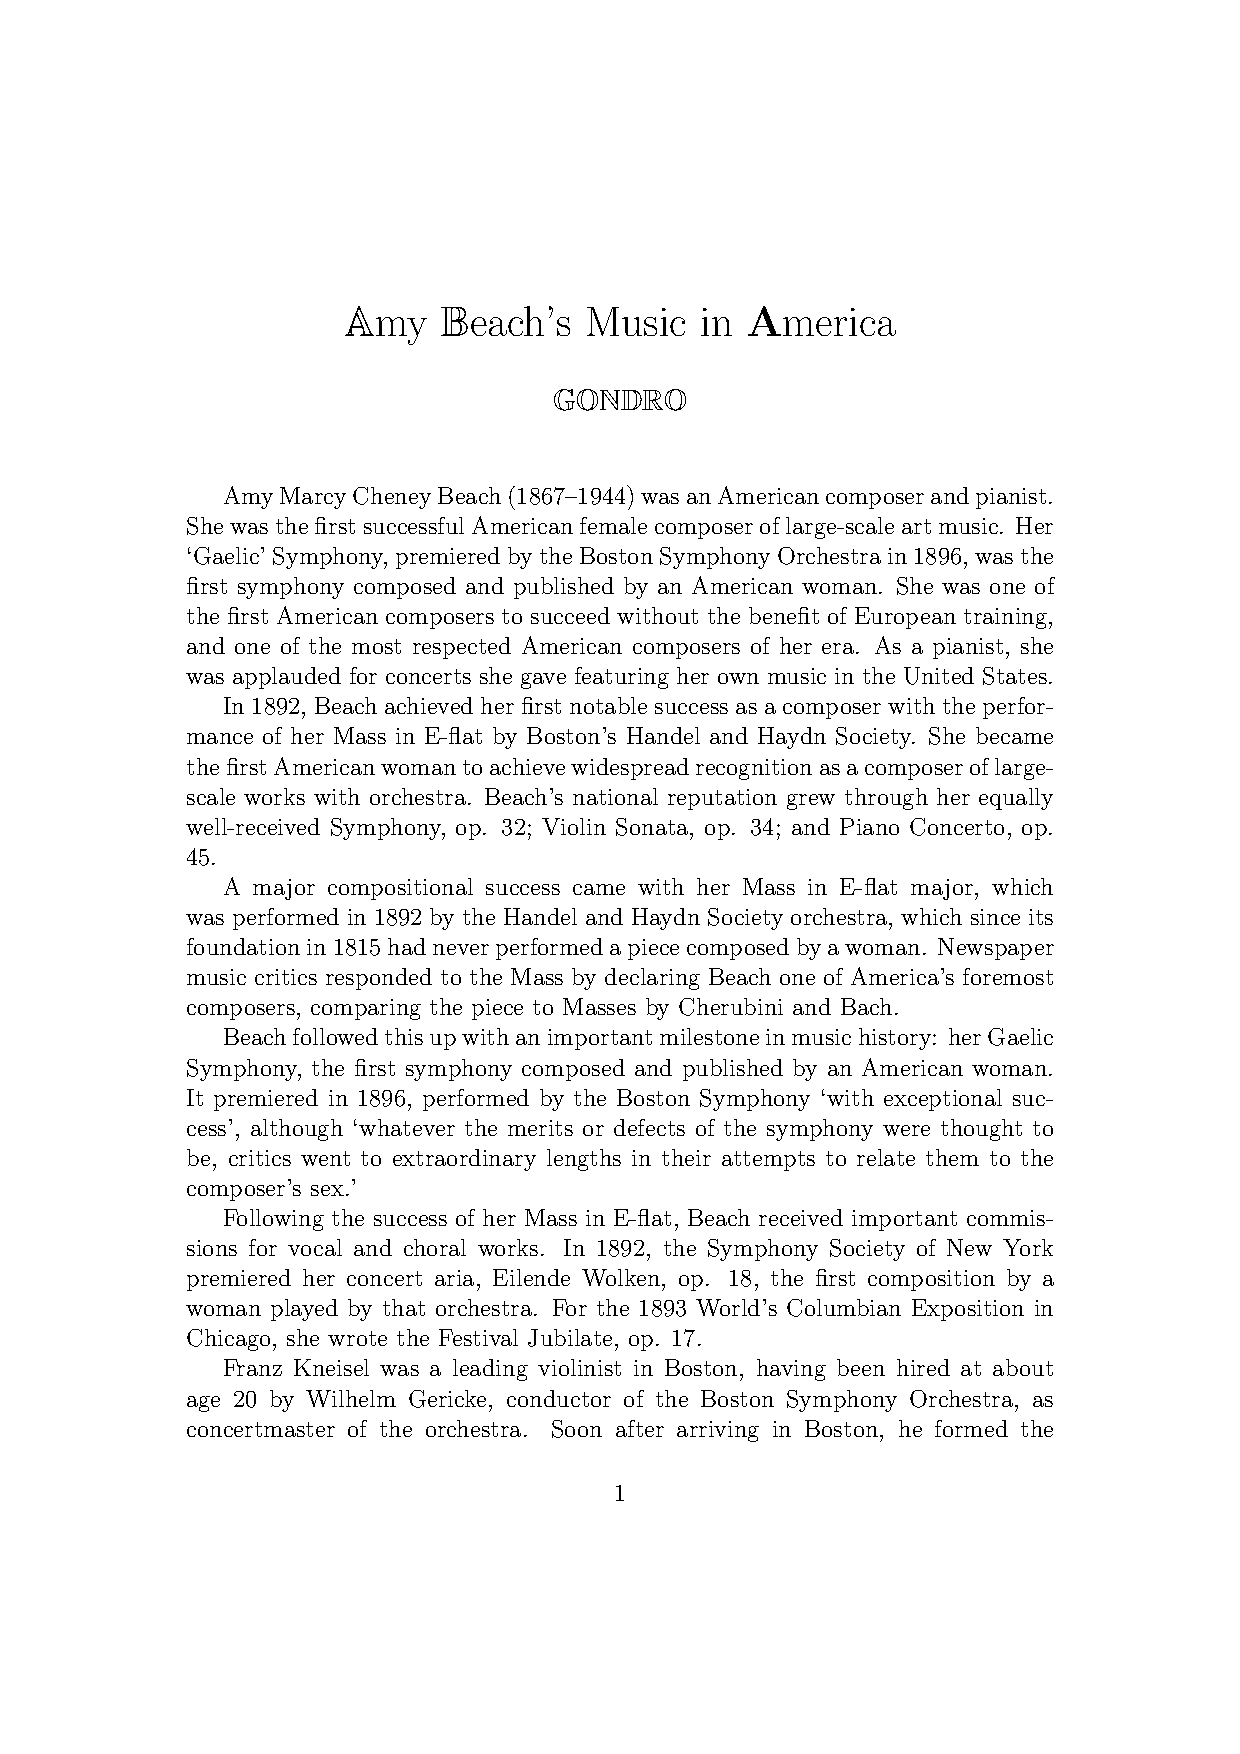
\includegraphics[width=.9\textwidth]{~/Pictures/amy.jpg}
\caption{This is $\mathbb A$my}
\end{figure}
\end{document}
